\section{Methodology: Quasielastic neutrino-nucleus cross sections}
\subsection{The nuclear model problem}
Currently there is no generally accepted model for calculating neutrino-nucleus interaction cross sections, applicable in a wide energy range from threshold to ultrahigh values. The importance of the choice of nuclear physics model for neutrino oscillations is considered in the work by Meloni and Martini~\cite{Meloni:2012fq}, where the results of the experiment T2K~\cite{Abe:2011sj,Abe:2012gx} retrieves the value of the neutrino mixing parameters with using conventional Relativistic Fermi gas model (RFG), as well as MECM model~\cite{Martini:2009uj}. The most striking difference is observed for the angle $\theta_{13}$: $\sin^{2}2\theta_{13}^{\textrm{RFG}}=0.138^{+0.031}_{-0.041}$ is approximately $1.5$ times bigger than $\sin^{2}2\theta_{13}^{\textrm{MECM}}=0.092^{+0.030}_{-0.052}$.

All of experimantal data mentioned in Introduction have been obtained by using RFG model. Applying another model could essentially modify extracted values including nucleon axial mass. Figure~\ref{MiniBooNE} demonstrates that nuclear model of Martini~\textit{et al.} can describe MiniBooNE data~\cite{AguilarArevalo:2010zc} \textbf{with $M_{A}=1.03$\,GeV}~\cite{Martini:2011wp}. At high energies nuclear effects are less important, that explains good agreement between experimental data and RFG model \textbf{with $M_{A}=1.012\pm{0.031}$\,GeV}~\cite{Kuzmin:2014}. Hydrogen and deuterium calculations don't use nuclear model at all and \textbf{gives us $M_{A}=1.026\pm{0.031}$\,GeV}~\cite{Kuzmin:2014}. $M_{A}$ extracted in both these cases are consistent with each other and with result of Martini~\textit{et al.}. K2K and T2K experiments that are not agree with $M_{A}\sim1$\,GeV, deal with lower neutrino energies too. The natural conclusion is that RFG model used for data processing in experiments does not work at low energies.

The problem is that there is no nuclear model which works properly for all energies. Therefore, even in case the correct value of the axial mass was known, using it with wrong nuclear model could not describe experimental data on quasielastic cross sections and would lead to errors in predictions.

\subsection{The effective axial mass approach}
Phenomenological solution of this problem is as follows. As we know, using RFG model with different values of $M_{A}$ can give a good description of experimental data obtained in different energy ranges. Thus, we propose to continue using this model but modify the axial form factor to compensate nuclear effects in the low-energy region. For this parametrization we need to introduce the variable effective axial mass as a function of neutrino energy and use it instead of conventional constant $M_{A}$. Of course, modified functions $F_{A}^\mathrm{eff}(Q^{2},E_{\nu})$, $F_{P}^\mathrm{eff}(Q^{2},E_{\nu})$, which defined by~(\ref{formfactors}) with $M_{A}$ replaced by $M_{A}^\mathrm{eff}$, are no longer axial-vector and pseudoscalar form-factors.

Figure~\ref{MA_QES_eff} demonstrates how one can fit experimental data to get the $M_{A}^\mathrm{eff}$. We chose for parameterization a simple form:
\begin{equation}
M_{A}^\mathrm{eff}=M_{0}\left(1+\frac{E_{0}}{E_{\nu}}\right).
\end{equation}
Global analysis of the experimental data on total and differential quasielastic neutrino cross-sections gives us the following values of parameters:
\begin{equation}
M_{0}=1.019\pm0.027\pm0.032\,\mathrm{GeV},E_{0}=0.327\tbinom{+0.060}{-0.056}\tbinom{+0.072}{-0.067}\,\mathrm{GeV},
\end{equation}
where $1\sigma$ and $2\sigma$ errors are shown.

\begin{figure}[htb!]
\begin{center}
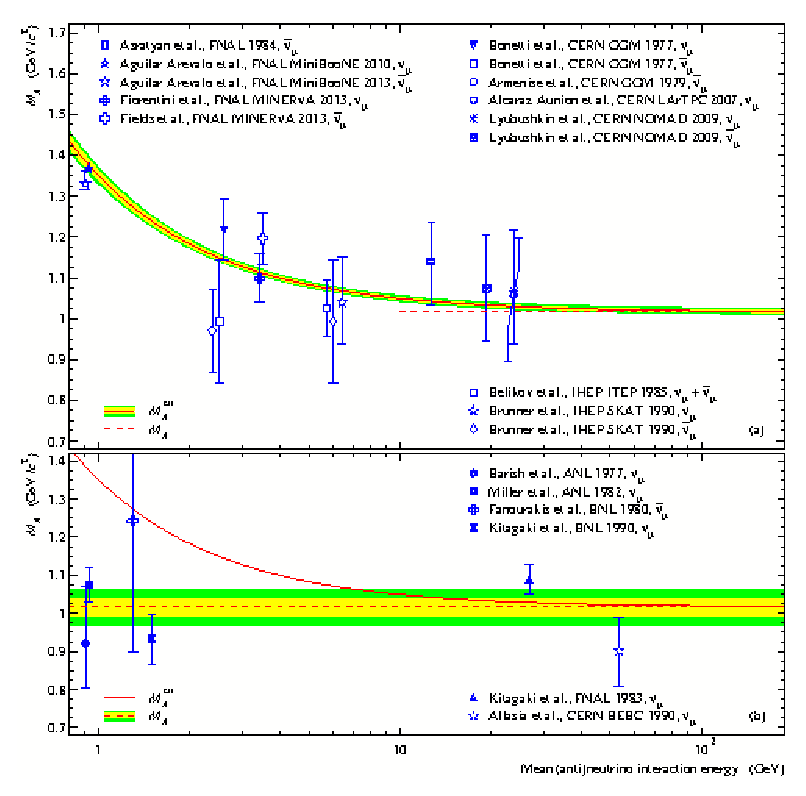
\includegraphics[width=0.6\textwidth]{./QES/MA_QES_eff.eps}
\caption{\label{MA_QES_eff}Fitting experimental data for $M_{A}^\mathrm{eff}$ parameterization. Only selected data are shown}
\end{center}
\end{figure}

In Fig.~\ref{TotalCS} it is shown, that data obtained in experiments with hydrogen and deuterium do not contradict with the best-fit constant axial mass. But MiniBooNE and, for example, NOMAD datasets are not consistent in any constant $M_{A}$ hypothesis. On the contrary, applying the offered $M_{A}^\mathrm{eff}$ gives a good description of these experiments. Please, pay attention on the fact that the flux energy peak of NO$\nu$A experiment lays between their studied areas as well as energy range of most of the fully-contained events in Super-Kamiokande.
